\documentclass[unicode,11pt,a4paper,oneside,numbers=endperiod,openany]{scrartcl}

% Required package
\usepackage{amssymb}
\usepackage{graphicx}
\usepackage{amsmath}
\usepackage{matlab-prettifier}
\usepackage{float}
\usepackage[export]{adjustbox}
\usepackage{multirow}
\usepackage{booktabs}

\renewcommand{\thesubsection}{\arabic{subsection}}

% vector shortcut
\newcommand{\myvec}[1]{\begin{bmatrix} #1 \end{bmatrix}}
\newcommand{\myex}[1]{\begin{equation*}\begin{aligned} #1 \end{aligned}\end{equation*}}
%\newcommand{\myexthreeA}{\myvec{2 & 0 \\ 0 & 2\mu}}
\newcommand{\myFigureEnergy}[3]{
    \begin{figure}[h]
    \centering
    \caption{#1}
    \label{#2}
    \includegraphics[width=\paperwidth, trim={9cm 0cm -2cm 0cm}]{./figures/#3}
    \end{figure}
}
\newcommand{\myFigureComparison}[4]{
    \begin{figure}[H]
    \centering
    \caption{#1}
    \label{#2}
    \includegraphics[width=.2\paperwidth, trim={8.5cm 0cm 0.5cm 0cm}]{./figures/#3}
    \includegraphics[width=.2\paperwidth, trim={0.5cm 0cm 8.5cm 0cm}]{./figures/#4}
    \end{figure}
}

\usepackage{ifthen}
\usepackage[utf8]{inputenc}
\usepackage{graphics}
\usepackage{graphicx}
\usepackage{hyperref}
\usepackage{amsmath}

\pagestyle{plain}
\voffset -5mm
\oddsidemargin  0mm
\evensidemargin -11mm
\marginparwidth 2cm
\marginparsep 0pt
\topmargin 0mm
\headheight 0pt
\headsep 0pt
\topskip 0pt        
\textheight 255mm
\textwidth 165mm

\newcommand{\duedate} {}
\newcommand{\setduedate}[1]{%
\renewcommand\duedate {\textbf{Due date:}~ #1}}
\newcommand\isassignment {false}
\newcommand{\setassignment}{\renewcommand\isassignment {true}}
\newcommand{\ifassignment}[1]{\ifthenelse{\boolean{\isassignment}}{#1}{}}
\newcommand{\ifnotassignment}[1]{\ifthenelse{\boolean{\isassignment}}{}{#1}}

\newcommand{\assignmentpolicy}{
\begin{table}[h]
\begin{center}
\scalebox{0.8} {%
\begin{tabular}{|p{0.02cm}p{16cm}|}
\hline
&\\
\multicolumn{2}{|c|}{\Large\textbf{Numerical Computing 2023 ---  Submission Instructions}}\\
\multicolumn{2}{|c|}{\large\textbf{(Please, notice that following instructions are mandatory: }}\\
\multicolumn{2}{|c|}{\large\textbf{submissions that don't comply with, won't be considered)}}\\
&\\
\textbullet & Assignments must be submitted to \href{https://www.icorsi.ch/course/view.php?id=14666}{iCorsi} (i.e. in electronic format).\\
\textbullet & Provide both executable package and sources (e.g. C/C++ files, MATLAB). 
If you are using libraries, please add them in the file. Sources must be organized in directories called:\\
\multicolumn{2}{|c|}{\textit{Project\_number\_lastname\_firstname}}\\
& and  the  file must be called:\\
\multicolumn{2}{|c|}{\textit{project\_number\_lastname\_firstname.zip}}\\
\multicolumn{2}{|c|}{\textit{project\_number\_lastname\_firstname.pdf}}\\
\textbullet &  The TAs will grade your project by reviewing your project write-up, and looking at the implementation you attempted, and benchmarking your code's performance.\\

\textbullet & You are allowed to discuss all questions with anyone you like; however: (i) your submission must list anyone you discussed problems with and (ii) you must write up your submission independently.\\
\hline
\end{tabular}
}
\end{center}
\end{table}
}
\newcommand{\punkte}[1]{\hspace{1ex}\emph{\mdseries\hfill(#1~\ifcase#1{Points}\or{Points}\else{Points}\fi)}}


\newcommand\serieheader[6]{
\thispagestyle{empty}%
\begin{flushleft}

\includegraphics[width=0.45\textwidth]{CI_logo}
\end{flushleft}
  \noindent%
  {\large\ignorespaces{\textbf{#1}}\hspace{\fill}\ignorespaces{ \textbf{#2}}}\\ \\%
  {\large\ignorespaces #3 \hspace{\fill}\ignorespaces #4}\\
  \noindent%
  \bigskip
  \hrule\par\bigskip\noindent%
  \bigskip {\ignorespaces {\Large{\textbf{#5}}}
  \hspace{\fill}\ignorespaces \large \ifthenelse{\boolean{\isassignment}}{\duedate}{#6}}
  \hrule\par\bigskip\noindent%  \linebreak
 }

\makeatletter
\def\enumerateMod{\ifnum \@enumdepth >3 \@toodeep\else
      \advance\@enumdepth \@ne
      \edef\@enumctr{enum\romannumeral\the\@enumdepth}\list
      {\csname label\@enumctr\endcsname}{\usecounter
        {\@enumctr}%%%? the following differs from "enumerate"
	\topsep0pt%
	\partopsep0pt%
	\itemsep0pt%
	\def\makelabel##1{\hss\llap{##1}}}\fi}
\let\endenumerateMod =\endlist
\makeatother




\usepackage{textcomp}





\begin{document}


\setassignment
\setduedate{Friday, 12 April 2024, 12:00 AM}

\serieheader
{Optimization Methods}
{2024}
{\textbf{Student:} Jeferson Morales Mariciano \\\\}
{\textbf{Discussed with:} Leonardo Birindelli}
{Assignment 2}{}
\newline

%\assignmentpolicy


% EXERCISE 1 %%%%%%%%%%%%%%%%%%%%%%%%%%%%%%%%%%%%%%%%%%%%%%%%%%%%%%%%%%%%%%%%%%%%%%%%%%%%%%%%%%%%%%
\section*{Exercise 1}
Considering the highly non-linear Rosenbrock's function:
\begin{equation} \label{eq:rosenbrock}
    f(x, y) := (1 - x)^2 + 100(y - x^2)^2 
\end{equation}

\subsection*{1, 2, 3}
Implement in MATLAB two functions: 
Newton's method (Newton.m), Steepest descent (Gradient) method (GD.m).
Both methods can be run with backtracking algorithm (backtracking.m) with step size $\beta = 1$. 
Use the following values for the backtracking parameters: 
$\tilde{\alpha} = 1, \rho = 0.9$. 
You can choose the parameter $c_1 \in [0.5, 10^{-4}]$.

Minimize the Rosenbrock's function \ref{eq:rosenbrock} 
by using the Steepest Descent (Gradient) method with backtracking and fixed step size $\beta = 1$. 
Use starting value $x_0 = (0, 0)$, 
maximum number of iterations $N = 50000$ and tolerance $TOL = 10^{-6}$.

Minimize the Rosenbrock's function \ref{eq:rosenbrock} 
by using Newton method with backtracking and fixed step size $\beta = 1$. 
Use same parameters as for SD.
\\\newline
Matlab scripts are provided in \textit{/code} folder.
The 2 main files to run are: \textit{GD.m, Newton.m}.
They handle both computations and visualization of the Rosenbrock's function with the corresponding methods.

\subsection*{4, 5, 6}
Plot the obtained iterates on the energy landscape in 2D.
Analyze convergence behaviour of the methods by plotting the gradient norm and the function
value at each iteration.
Compare and comment on the the performances of the different methods.
\\\newline
\myFigureComparison
    {Convergence comparison between methods with Backtracking}
    {fig:ex1-convergence-comparison-backtracking}
    {ex1-sd-backtracking-convergence.eps}
    {ex1-newton-backtracking-convergence.eps}

\myFigureEnergy
    {Visualization of Steepest Descent with Backtracking}
    {fig:ex1-sd-backtracking-energy}
    {ex1-sd-backtracking-energy.eps}

\myFigureEnergy
    {Visualization of Newton Method with Backtracking}
    {fig:ex1-newton-energy-backtracking}
    {ex1-newton-backtracking-energy.eps}

\myFigureComparison
    {Convergence comparison between methods without Backtracking}
    {fig:ex1-convergence-comparison}
    {ex1-sd-convergence.eps}
    {ex1-newton-convergence.eps}

\myFigureEnergy
    {Visualization of Steepest Descent without Backtracking}
    {fig:ex1-sd-energy}
    {ex1-sd-energy.eps}

\myFigureEnergy
    {Visualization of Newton Method without Backtracking}
    {fig:ex1-newton-energy}
    {ex1-newton-energy.eps}

Chosen value for parameter $c_1 = 1e-4$. 
Both methods are run with backtracking algorithm with step size $\beta = 1$.
For the Newton's method without backtracking, 
when it reaches the local minimum at $x^* = (1, 1)$,
in order to plot it logarithmically the value $0 \mapsto EPS$ with $EPS = 2.2204e-16$ 
in order to visualize symbolically the convergence to $0$.
\newline

\textbf{Convergence behavior:}
Newton method converges faster than Steepest Descent, 
regardless of the usage of the backtracking algorithm to compute the step length $\alpha$.
The Steepest Descent method converges after 21103 iterations with backtracking 
as in Figure \ref{fig:ex1-sd-backtracking-energy}
and it does not converge at all without backtracking as Figure \ref{fig:ex1-sd-energy} show:
notice that the energy landscape is not shown due to the linear search going out of bounds of the rendered 
part of the Rosenbrock function. 
Meanwhile, the Newton method converges after 13 iterations with backtracking 
as in Figure \ref{fig:ex1-newton-energy-backtracking} and in 3 iterations, 
so even less, without backtracking as in Figure \ref{fig:ex1-newton-energy}.
The gradient norm and the function value at each iteration are plotted for both methods 
with and without the Backtracking algorithm in the before-mentioned figures.
Such behavior is explained because the Newton method uses the Hessian matrix to compute the step direction
and will converge quadratically for all $x$ in the neighborhood of the solution point $\mathcal{N}(x^*)$ 
such that $\nabla f(x^*)$ is positive definite,
thus the Hessian matrix $H_f(x) = \nabla^2 f(x)$ is also positive definite.
\newline

\textbf{Performances of methods:}
in addition, the convergence comparison between methods with and without backtracking
plotting the input values $x_1, x_2$ of the function along iterations converging to the local minima 
is shown in Figure \ref{fig:ex1-convergence-comparison-backtracking} for backtracking comparison, 
and Figure \ref{fig:ex1-convergence-comparison} for $\beta = 1$ fixed step length size.
The steepest descent is a first-order method and its convergence is linear from Theorem 3.3.
Its characterized by zigzagging behavior when searching for the local minima.
On the other hand, Theorem 3.5 states that the Newton method is a second-order method, 
its convergence is quadratic and its sequence of gradient norms converges quadratically to 0.
For higher dimension and orders of convergences, the Newton method is faster and suggested.
Remember that the Newton method is not always the best choice, 
since it requires the computation of the Hessian matrix which is computationally expensive $O(n^3)$ 
because needs to compute the second derivative and solve a linear system. 
Hence, beware of Newton's method, specially for large scale problems 
and keep in mind that the Hessian matrix is not always positive definite, 
meaning it could not even yield a descent direction. 
\clearpage

% EXERCISE 2 %%%%%%%%%%%%%%%%%%%%%%%%%%%%%%%%%%%%%%%%%%%%%%%%%%%%%%%%%%%%%%%%%%%%%%%%%%%%%%%%%%%%%%
\section*{Exercise 2}

\subsection*{1, 2}
Implement the BFGS method (BFGS.m) with backtraking for the step size $\beta$. 
Test your implementation by minimizing the Rosenbrock's function. 
Use starting values $x_0 = (0, 0)$, 
$H_0 = I$, 
maximum number of iterations $N = 500$ and tolerance $TOL = 10^{-6}$.
\\\newline
Matlab scripts are provided in \textit{/code} folder.
The main file to run is \textit{BFGS.m}.
It handles both computations and visualization of the Rosenbrock's function with the corresponding method.

\subsection*{3, 4}
Plot the obtained iterates on the energy landscape in 2D.
Analyze convergence behaviour of the methods by plotting the gradient norm and the function
value at each iteration.

\myFigureEnergy
    {Visualization of BFGS}
    {fig:ex2-bfgs-energy}
    {ex2-bfgs-energy.eps}

\begin{figure}[H]
    \centering
    \caption{Convergence of BFGS with Backtracking}
    \label{fig:ex2-bfgs-convergence}
    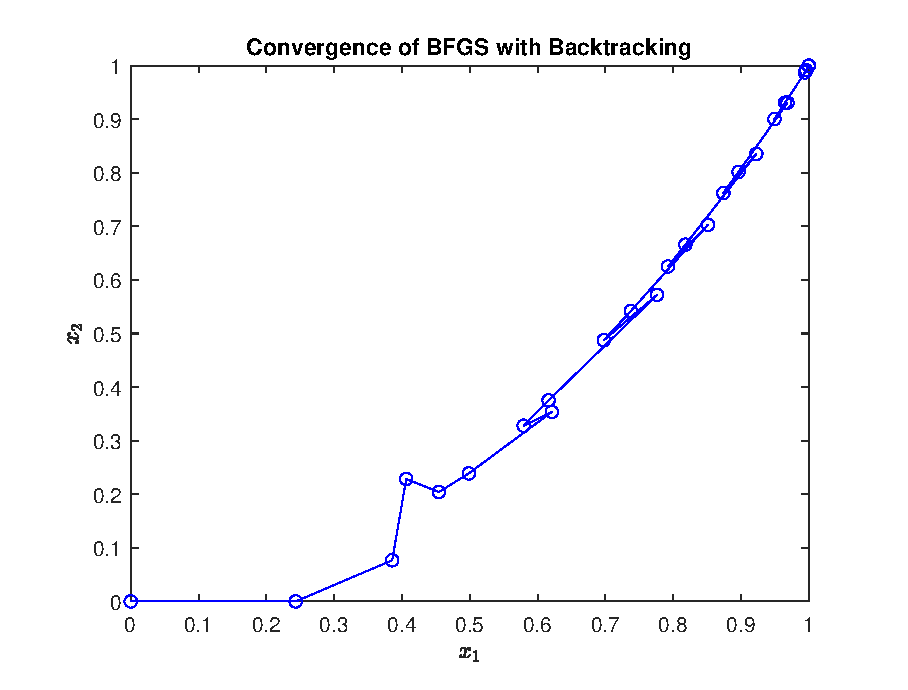
\includegraphics[width=.6\textwidth, trim={0cm 0cm 0cm 0cm}, clip]{./figures/ex2-bfgs-convergence.eps}
\end{figure}

The plots regarding the energy landscape both 3D and 2D together with 
the convergence behavior of the BFGS method with respect to gradient norms and function values 
are visualized in Figure \ref{fig:ex2-bfgs-energy}.
The BFGS method convergence stop because it reaches a local minima approximation 
below the tolerance $TOL = 10^{-6}$ when computing the norm of the gradient $\nabla f(x^*)$.

\subsection*{5}
Produce a table in which you compare the number of iterations required by BFGS, 
by Newton's method (with backtracking) and by Steepest descent method (with backtracking). 
You can use the results from the previous exercise. 
Comment the results by comparing the different methods.

\begin{table*}[h] 
    \centering
    \caption{Comparison of Iterations for Rosenbrock's Function}
    \label{tab:ex2-iterations-comparison}
    \begin{tabular}{@{}ccc@{}}
        \toprule
        Newton & BFGS & Steepest Descent \\
        \midrule
        13  & 27 & 21103 \\
        \bottomrule
    \end{tabular}
\end{table*}

In Table \ref{tab:ex2-iterations-comparison}, it is shown the number of iterations required by
the Steepest Descent, Newton and BFGS methods to minimize the Rosenbrock's function 
in ascending order of convergence.
The iteration counter starts at 1, so not entering the loop is considered as 1 iteration.
Order of convergence speed: Newton, BFGS, Steepest Descent.
The reason relies on the order of the method dictating the convergence rate:
steepest descent convergence rate is linear, 
Newton is quadratic 
and BFGS which is a quasi-Newton method with a superlinear convergence rate.
The BFGS has such convergence rate because it approximates the inverse Hessian matrix $H_k$ 
which combines the most recently observed information about the objective function 
with the existing knowledge embedded in the approximation $H_{k-1}$.
It is suggested to use such quasi-newton method for large scale problems instead of the Newton method
to avoid the need to compute second derivatives and solve linear systems.
\clearpage

% EXERCISE 3 %%%%%%%%%%%%%%%%%%%%%%%%%%%%%%%%%%%%%%%%%%%%%%%%%%%%%%%%%%%%%%%%%%%%%%%%%%%%%%%%%%%%%%
\section*{Exercise 3}
Let 
$f : \mathbb{R} \rightarrow \mathbb{R}$ 
be given by 
$f = \frac{1}{2} x^T Ax - b^T x$ 
with $A$ symmetric positive definite. 
How many iterations does the SD method take to minimize the function $f$ 
if we use the optimal step length? 
Please, prove your answer.
\\\newline
From Theorem 3.3, when the steepest descent method with exact line searches $\alpha_{opt}$:
\myex{
    x_{k+1} = x_k 
        - \underbrace{
            \left( 
                \frac{\nabla f_k^T \nabla f_k}{\nabla f_k^T Q \nabla f_k} 
            \right)
        }_{\alpha_{opt}} 
        \nabla f_k 
        \;\;\;\;\;\text{ where Q is SPD} 
}
is applied to the strongly convex quadratic function of the form:
\myex{
    f(x) = \frac{1}{2} x^T Q x - b^T x
    \;\;\;\;\;\text{ where Q is SPD} 
}
as the requested function $f$ from the exercise is, 
the error norm:
\myex{
    \frac{1}{2} ||x - x^*||_Q^2 = f(x) - f(x^*)
}
satisfies:
\myex{
    & ||x_{k+1} - x^*||_Q^2 
    \leq 
    \left( 
        \frac{\lambda_{n} - \lambda_{1}}{\lambda_{n} + \lambda_{1}} 
    \right)^2 
    ||x_k - x^*||_Q^2
    \\
    & \text{ with }
    0 < \lambda_1 \leq \lambda_2 \leq \ldots \leq \lambda_n,\;
    \lambda \in \Lambda = spectrum(Q)
}
The special case of the last formula see that convergence is achieved in one iteration
if all eigenvalues are equal 
$\lambda_i = \lambda_j \text{ for } i \neq j,\; \forall \lambda \in \Lambda = spectrum(Q)$.
\myex{
    \underbrace{||x_{k+1} - x^*||_Q^2}_{||\cdot||^2 \geq 0} 
    \leq 0
}
In this case, $Q$ is a multiple of the identity matrix $I$, 
so the contours are circles and the steepest descent direction always points at the solution.

\end{document}
